\documentclass[a4paper]{article}
\usepackage[T2A]{fontenc}
\usepackage[utf8]{inputenc}
\usepackage[english,bulgarian]{babel}
\usepackage{graphicx}
\usepackage{url}
\usepackage{textcomp}
\usepackage{amsmath}
\usepackage{amsfonts}
\usepackage{amssymb}
\usepackage{tabularx}
\usepackage{array}
\usepackage[margin=1.5in]{geometry}
\usepackage[unicode]{hyperref}

\usepackage{fancyhdr}
\setlength{\headheight}{15pt}
 
\pagestyle{fancyplain}

\usepackage{listings}
\lstset{language=Java,captionpos=b,
tabsize=4,frame=lines,
basicstyle=\small\ttfamily,
keywordstyle=\color{blue},
commentstyle=\color{gray},
stringstyle=\color{violet},
breaklines=true,showstringspaces=false}


\addto\captionsbulgarian{%
  \renewcommand{\contentsname}%
    {Содржина}%
  \renewcommand{\tablename}%
    {Табела}%
  \renewcommand{\figurename}%
    {Слика}%
  \renewcommand{\bibname}%
    {Библиографија}%
  \renewcommand{\listfigurename}%
    {Листа на слики}%
  \renewcommand{\listtablename}%
    {Листа на табели}%
}

\rhead{\textsc{Напредно програмирање}}
\chead{}
\lhead{Аудиториски вежби 1}
\lfoot{}
\cfoot{\thepage}
\rfoot{}
\usepackage{fancyvrb}
\usepackage{xcolor}

\usepackage{textcomp}

\begin{document}


\section{Што е Eclipse?}
Eclipse претставува интегрирана околина за развој (IDE) за програмскиот јазик
Java. Денес претставува водечка околина за развој за Java со опфатен дел од
пазарот од приближно 65\%.

Eclipse е создаден од Open Source заедницата и се користи во повеќе различни
области, пр. како развојна околина за Java или Android апликации.
Развојот на Eclipse датира од 2001.

Eclipse Open Source заедницата има преку 200 Open Source проекти во
повеќе различни аспекти од развојот на софтвер.

Сите Eclipse проекти ги води \emph{Eclipse Foundation}. Тоа е не профитна
организација, поддржана од своите членови со цел да хостира Eclipse Open Source
проекти и да помага во созревањето на Open Source заедницата и како
комплементарен екосистем на производи и сервиси.

Eclipse IDE може да се прошири со додатни софтверски компоненти кои се
нарекуваат \emph{plug-ins}. Притоа постојат повеќе Open Source проекти од
различни компании кои го имаат проширено Eclipse IDE.

Eclipse може да се користи и како основа за креирање на апликации со помош на
Eclipse Rich Client Platform (\emph{Eclipse RCP}) за апликации.

\section{Eclipse Public License}

\emph{Eclipse Public License} (EPL) е Open Source софтверска лиценца која ја
користи \emph{Eclipse Foundation} за нејзиниот софтвер. EPL е дизајнирана да
биде соодветна за бизнисите со тоа што EPL лиценцираните програми може да се
користат, модификуваат, копираат и дистрибуираат слободно и без да се плаќа.


\section{Инсталација на Eclipse}

\subsection{Java побарување на Eclipse}

Eclipse има потреба од инсталирана Java Runtime околина, односно минмум Java
5 за да се извршува. Притоа препорачливо е користење на Java верзија 6 или
повисока.

Eclipse IDE содржи сопствен Java компајлер. За компајлирање изворен
код надвор од Eclipse потребни се  \emph{Java Development Tools}.

\subsubsection{Инсталација на Java}

Java можеби е веќе инсталирана на вашата машина. Ова може да се провери со
отворање на конзола (ако сте на Windows: \texttt{Win+R}, внесете \texttt{cmd} и
притиснете \texttt{Enter}) и впишување на следната команда:

\begin{verbatim}
java -version 
\end{verbatim}

Ако Java е соодветно инсталирана, треба да видите информации за тоа. Ако
командната линија врати резултат дека програмата не може да се најде, треба да
инсталирате Java.

Google пребарување за ``How to install JDK on \emph{\texttt{YOUR\_OS}}'' треба
да врати резултати со линкови со помош. Заменете го \emph{\texttt{YOUR\_OS}} со
вашиот оперативен систем, пр. ~Windows, Ubuntu, Mac OS X, итн.

\subsection{Download Eclipse}

Eclipse.org веб сајтот содржи запакувани инсталации на Eclipse дистрибуции.

Симнете го \emph{Eclipse IDE for Java Developers} пакетот од следното URL:

\begin{verbatim}
http://www.eclipse.org/downloads 
\end{verbatim}

На следните слики е прикажан сајтот на Eclipse за симнување на за на Linux
систем.

\begin{figure}[htbp]
\centering
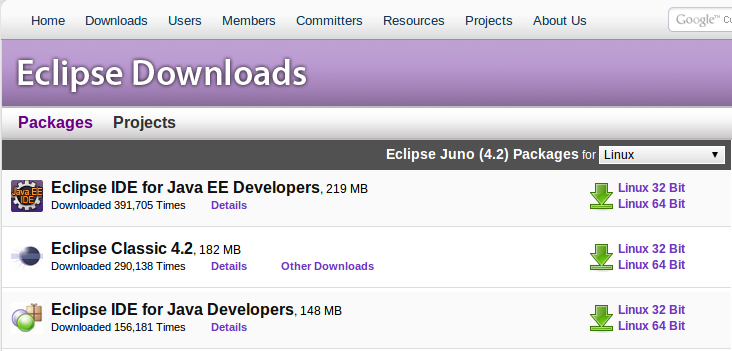
\includegraphics[scale=0.5]{images/download}
\caption{Eclipse Download страница}
\end{figure}

Содржината на симнувањето е \texttt{.zip} датотека.

\subsection{Инсталација на Eclipse}

Откако ќе ја симнете \texttt{.zip} датотеката која ја содржи Eclipse
дистрибуцијата едниствено треба да ја отпакувате во посакуваниот локален
директориум.

Употеребете директориум во чија патека нема празни места, затоа што Eclipse
понекогаш има проблем со тоа.

По отпакувањето може да го користите Eclipse. Нема потреба од дополнителни
инсталации.

\section{Работа со Eclipse}

\subsection{Стартување Eclipse}

Стартувајте го Eclipse со двоен-клик на датотеката \texttt{eclipse.exe}
(Microsoft Windows) или \texttt{eclipse} (Linux / Mac) во директориумот кој го
отпакувавте Eclipse.

\begin{figure}[htb]
\centering
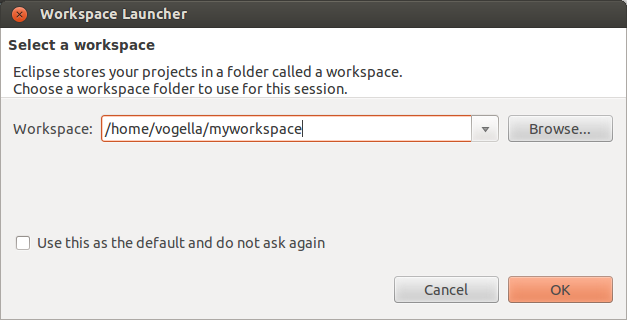
\includegraphics[scale=.5]{images/workspace}
\caption{Избор на Workspace}
\label{fig:workspace}
\end{figure}


Системот ќе побара да изберете \emph{workspace} (слика
\ref{fig:workspace}). \emph{Workspace} е местото каде што ќе работите. Изберете
празен директориум и притиснете на копчето OK.


Eclipse ќе се стартува и ќе прикаже Welcome страница. Затворете ја оваа
страница.

\begin{figure}
\centering
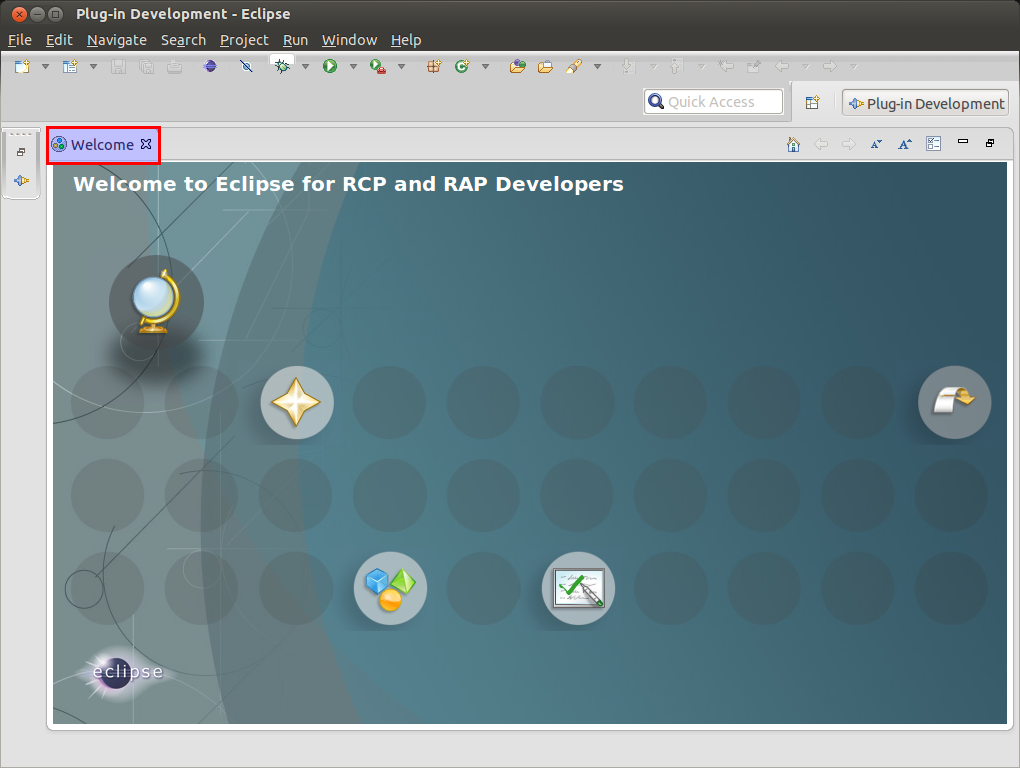
\includegraphics[width=\textwidth]{images/welcome}
\caption{Затворање на Eclipse welcome screen}
\end{figure}

Откако ќе го затворите почетниот екран треба да видите екран сличен на следниот:

\begin{figure}
\centering
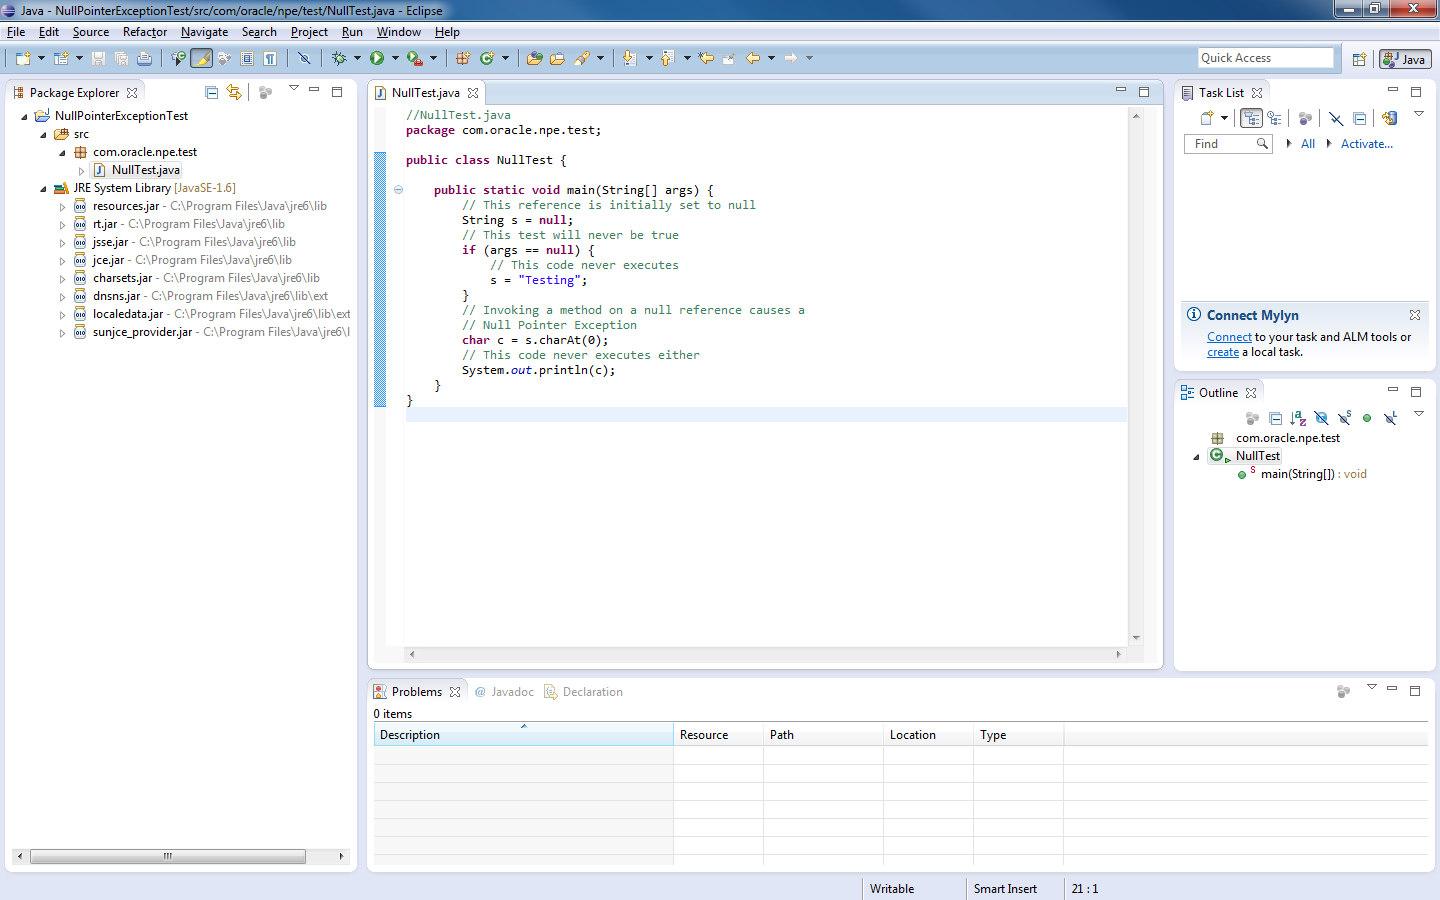
\includegraphics[width=\textwidth]{images/screen}
\caption{Почетен Eclipse поглед}
\end{figure}


\section{Преглед на Eclipse корисничкиот интерфејс}

Eclipse е составен од \emph{Perspectives}, \emph{Views} и \emph{Editors}.
\emph{Views} и \emph{Editors} се групирани во \emph{Perspectives}.

\hyperdef{}{workspace}{\subsection{Workspace}\label{workspace}}

\emph{Workspace} е физичката локација (патеката на датотеките) со кои работите.
Вашите проекти, изворни датотеки, слики и други артефакти може да се чуваат во
вашиот работен простор, но исто така може да референцирате и надворешни ресурси
(пр. проекти). 

Може да изберете работен простор на стартување на Eclipse или преку мени (File →
Switch Workspace → Others).

\hyperdef{}{parts}{\subsection{Parts}\label{parts}}

\emph{Parts} се компоненти од корисничкиот интерфејс кои овозможуваат да
навигирате и модификувате податоци. Вообичаено поделени во \emph{Views} и
\emph{Editors}.

\begin{figure}
\centering
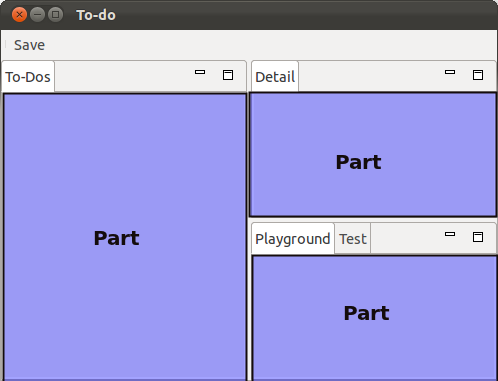
\includegraphics[scale=.5]{images/parts}
\caption{Eclipse апликација со неколку делови}
\end{figure}

Раздвојувањето на \emph{Views} и \emph{Editors} примарно не е базирано на
технички разлики, туку на различни концепти на користење и нивно уредување.

\emph{View} вообичаено се користи за работа со податоци, кои може да се во
хиерархиска структура. Ако податоците се променат преку \emph{View}, оваа
промена вообичаено директно се применува на податочната структура под неа.
\emph{View} понекогаш овозможува да се отвори \emph{Editor} за избрано множество
податоци.

Пример за \emph{View} е \emph{Java Package Explorer}, кој овозможува да се
прелистуваат датотеките во Eclipse проектите. Ако промените податоци во Package
Explorer, на пр. промените име на датотека, ова име директно се менува и во
податочниот систем.

\emph{Editors} вообичаено се употребуваат за менување единечен податочен
елемент, пр. датотека или податочен објект. За да се применат овие промени,
потребно е корисникот експлицитно да ја зачуваа содржината од едиторот.

\emph{Editors} традиционално се позиционирани во одредена област, наречена
\emph{editor area}.

\hyperdef{}{perspective}{\subsection{Perspective}\label{perspective}}

\emph{Perspective} е визуелен контејнер на множество од делови \emph{Parts}.
Eclipse IDE користи \emph{Perspectives} за да ги уреди \emph{Parts} за
различни задачи при развој. \emph{Perspectives} се менуваат преку менито Window
→ Open Perspective → Other (слика \ref{fig:perspective}).

Основните перспективи во Eclipse IDE се Java перспективата за развој и
перспективата Debug за дебагирање на Java апликации.

\begin{figure}[htb]
\centering
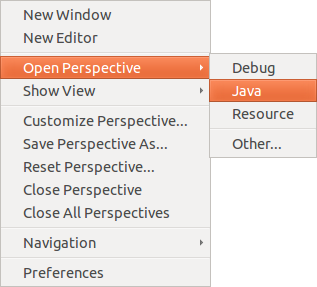
\includegraphics[scale=.5]{images/perspective}
\caption{Менување перспективи во Eclipse IDE}
\label{ref:perspective}
\end{figure}

Може да ги менувате позициите и содржината на деловите во \emph{Perspective} со
отварање и затворање или со едноставно уредување со влечење.

\begin{figure}[htb]
\centering
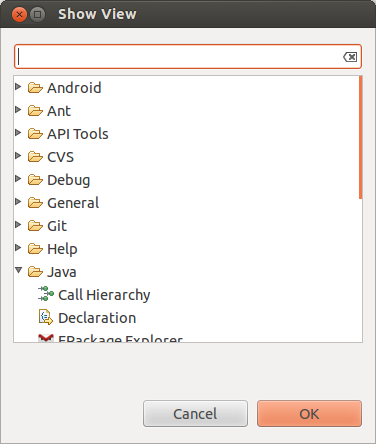
\includegraphics[scale=.5]{images/dialog}
\caption{Show View дијалог}
\label{fig:dialog}
\end{figure}

За да отворите нов \emph{Part} во вашата тековна \emph{Perspective} користете го
менито Window → Show View → Other. Следниот \texttt{Show View} (слика
\ref{fig:dialog}) дијалог ви овозможува да пребарувате одредени Parts.

\begin{figure}[htb]
\centering
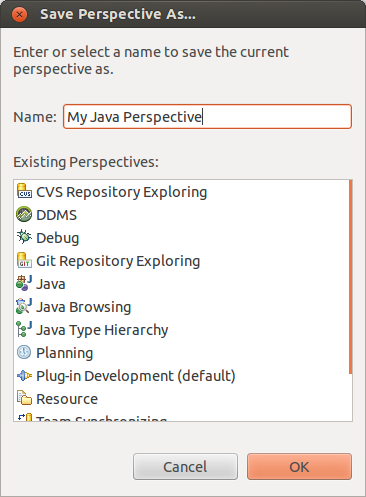
\includegraphics[scale=.5]{images/save-perspective}
\caption{Снимање на вашата перспектива конфигурација}
\label{fig:save}
\end{figure}

Во случаи кога сакате да ја ресетирате вашата тековна перспектива на нејзината
стандардна, можете преку менито Window → Reset Perspective.

Може да ја снимите вашата \emph{Perspective} преку Window → Save Perspective
As\ldots{} (слика \ref{fig:save}).

\section{Креирање на првата Java програма}

Во следните неколку чекори ќе го опишеме процесот на креирање едноставна и
минимална Java програма со користење Eclipse. Вообичаено во светот на
програмирањето оваа програма испишува ``Hello World'' во конзолата, но ние ќе ја
адаптираме да отпечати ``Hello Eclipse!'' стандардниот излез.

\subsection{Креирање проект}

Изберете од мениот File → New → Java project. Внесете
\texttt{edu.finki.np.hello} како име на проектот. Изберете ``Create separate folders for sources and class files''.

\begin{figure}
\centering
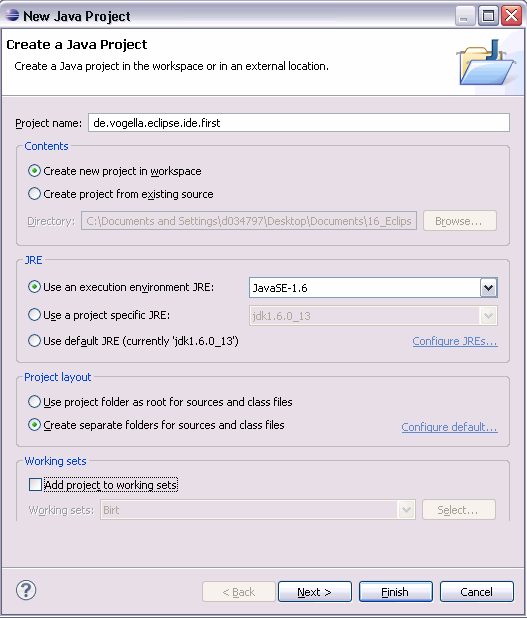
\includegraphics[scale=.5]{images/project}
\caption{Волшебникот за нов Java Project}
\end{figure}

Притиснете на копчето Finish за да го креирате проектот. Креиран е нов проект и
е прикажан како директориум. Отворете го \texttt{edu.finki.np.hello} и
прегледајте ја неговата содржина.

\subsection{Креирање пакети}

Во следниот чекор ќе креирате нов \texttt{package}. Добра конвенција е да
користите исто име за проектот и пакетот на највисоко ниво.

Да креирате пакет \texttt{edu.finki.np.hello}, изберете го фолдерот
\texttt{src} и со десен клик на него изберете New → Package.

\begin{figure}
\centering
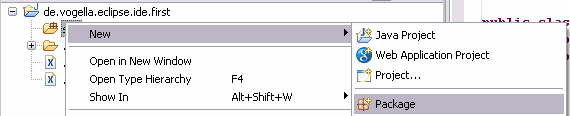
\includegraphics[scale=.5]{images/package}
\caption{Десен клик за креирање пакет}
\end{figure}

Внесете го името на новиот пакет во дијалогот.

\begin{figure}
\centering
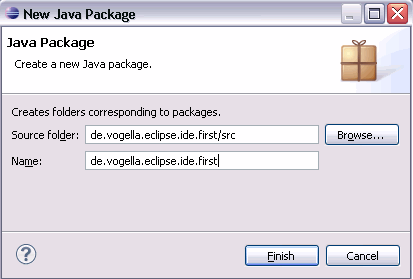
\includegraphics[scale=.5]{images/pkg_name}
\caption{Дијалог за креирање пакет}
\end{figure}

\subsection{Креирање Java класа}

Десен клик на пакетот и изберете New → Class.

\begin{figure}
\centering
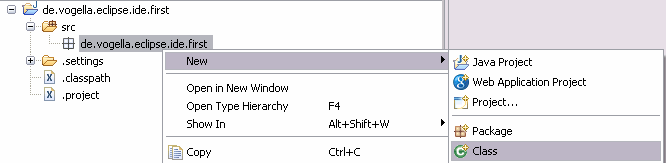
\includegraphics[scale=.5]{images/add-class}
\caption{Избор за креирање нова класа}
\end{figure}

Внесете \texttt{MyFirstClass} како име на класата и изберете го ``public static
void main (String{[}{]} args)''.

\begin{figure}
\centering
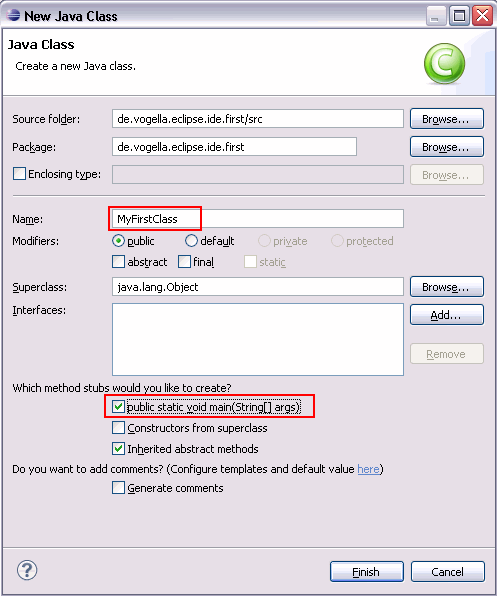
\includegraphics[scale=.5]{images/new-class}
\caption{Избор за креирање нова класа}
\end{figure}

Ова создава нова датотека и ја отвара во \emph{Editor} за Java изворни
датотеки. 

\begin{lstlisting}[language=Java]
package edu.finki.np.first;

public class MyFirstClass {

  public static void main(String[] args) {
    System.out.println("Hello Eclipse!");
  }

} 
\end{lstlisting}

\subsection{Извршување на проект во Eclipse}

За да го извршите кодот, со десен клик на вашата Java класа изберете Run-as →
Java application.

\begin{figure}
\centering
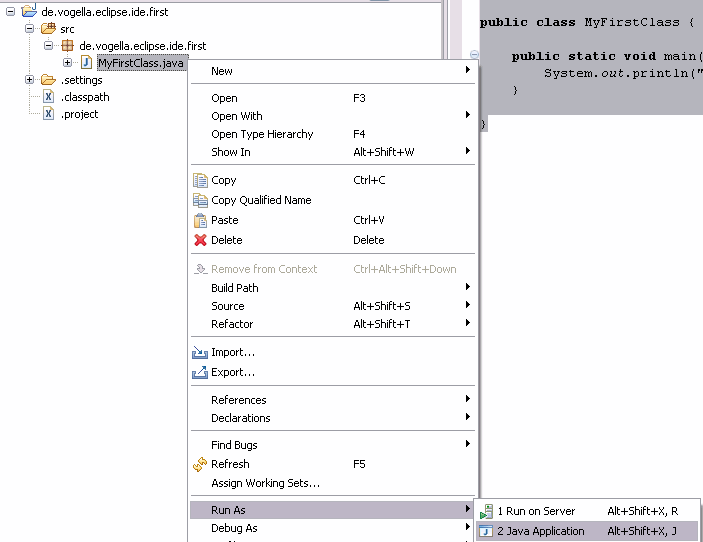
\includegraphics[scale=.5]{images/run}
\caption{Ивршување проект}
\end{figure}

Eclipse ќе ја изврши вашата Java програма. Треба да го видите следниот излез во
конзола \emph{View}.

\begin{figure}
\centering
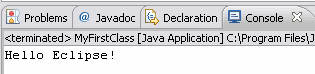
\includegraphics[scale=.5]{images/result}
\caption{Резултат од извршување на апликацијата}
\end{figure}

Честитки! Го креиравте вашиот прв Java проект, пакет и Java класа и ја извршивте
оваа програма во Eclipse.

\section{Извршување Java програма надвор од Eclipse}

\subsection{Креирање на jar датотека}

За да извршите Java програма надвор од Eclipse треба да ја експортирате како
\texttt{jar} датотека. \texttt{jar} датотека е стандарден формат за дистрибуција
на Java апликации.

Изберете го вашиот проект, десен клик и изберете \texttt{Export}.

\begin{figure}
\centering
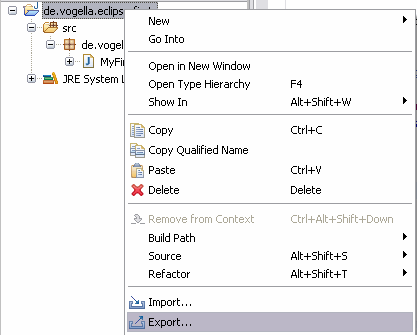
\includegraphics[scale=.5]{images/export}
\caption{Волшебник за експортирање на Java проект}
\end{figure}

Изберете JAR датотека, изберете next. Изберете го вашиот проект и изберете си
дестинација и име за jar датотеката. Пример \texttt{myprogram.jar}.

\begin{figure}
\centering
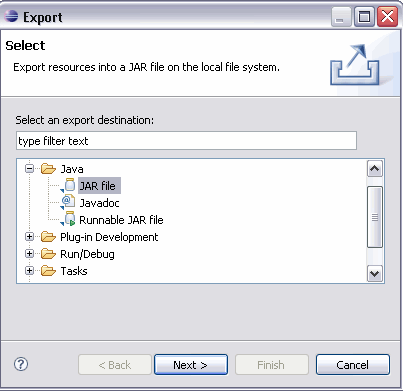
\includegraphics[scale=.5]{images/export-jar}
\caption{Волшебник за експортирање на Java проект, дел II}
\end{figure}

\begin{figure}
\centering
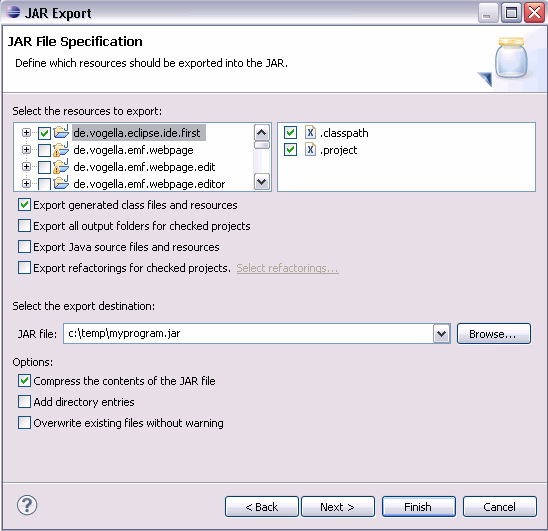
\includegraphics[scale=.5]{images/wizzard}
\caption{Волшебник за експортирање на Java проект, дел III}
\end{figure}

Честитки! 

\subsection{Извршете ја вашата програма надвор од Eclipse}

Отворете командна линија.

Променете ја вашата работна патека со испишување \texttt{cd path}. На пример
ако вашиот jar е лоциран во \texttt{c:\textbackslash{}temp} испишете \texttt{cd c:\textbackslash{}temp}.

За да ја извршите оваа програма треба да ја вклучите jar датотеката во вашиот
\texttt{classpath}. Со \texttt{classpath} се дефинираат сите Java класи кои се
овозможени во Java извршната околина. Може да додате \texttt{jar} датотека во
classpath со опцијата \texttt{-jar}.

\begin{verbatim}
java -classpath myprogram.jar edu.finki.np.first.MyFirstClass 
\end{verbatim}

Ако ја испиште точно наведената команда и се наоѓате во соодветнио директориум,
треба да видите порака ``Hello Eclipse!'' во конзолата.

\begin{figure}
\centering
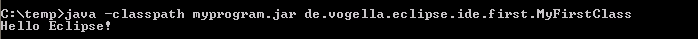
\includegraphics[scale=.5]{images/win}
\caption{Извршување апликација надвор од Eclipse}
\end{figure}

\section{Content Assist, Quick Fix и Class Navigation}

\subsection{Content assist}

Помошникот за содржина ви овозможува да добиете помош во самиот едитор. Може
да се повика со \textbf{Ctrl}+\textbf{Space}

На пример испишете \texttt{syso} во едиторот на Java изворен код и притиснете
\textbf{Ctrl}+\textbf{Space}. Ова ќе го замени \texttt{syso} со
\texttt{System.out.println("")}.

Ако имате референца кон објект, како на пример објектот \texttt{person} од типот
\texttt{Person} и сакате да ги видите неговите методи, испишете \texttt{person.}
и притиснете \textbf{Ctrl}+\textbf{Space}.

\begin{figure}
\centering
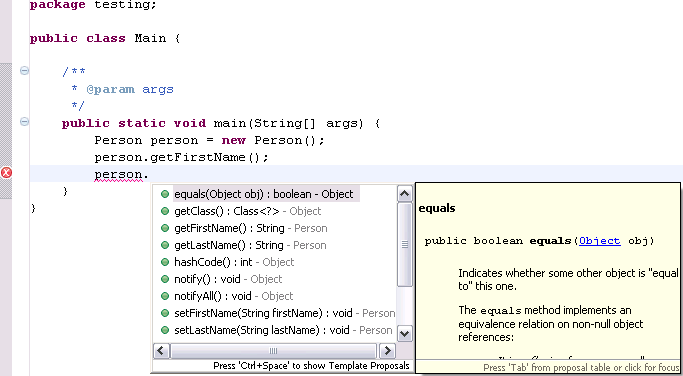
\includegraphics[scale=.5]{images/autocomplete}
\caption{Помошник во содржината}
\end{figure}

\subsection{Quick Fix}

Секогаш кога Eclipse детектира некаков проблем, ќе ве го подцрта проблематичниот
текст во едиторот. Изберете го овој текст и притиснете \textbf{Ctrl}+\textbf{1}
за да видите можни начини за да го решите овој проблем.

На пример напишете \texttt{myBoolean = true;} Ако myBoolean не е сѐ уште
дефинирана, Eclipse ќе ја означи како грешка. Изберете ја променливата и
притиснете \textbf{Ctrl}+\textbf{1}, Eclipse ќе ви предложи креирање на член или
локална променлива.

\begin{figure}
\centering
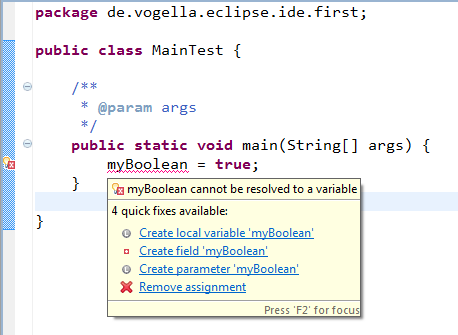
\includegraphics[scale=.5]{images/quick-fix}
\caption{Пример со користење Quickfix}
\end{figure}

Quick Fix е многу моќна алатка. Ви овозможува да креирате нови локални
променливи и членови, како и нови методи и класи. Исто така може да додава
try-catch изрази околу исклучоците, а може да извршува и доделување на
променливи, како и многу повеќе.

\section{Отворање класа}

Може да навигирате помеѓу класите во вашиот проект преку ``Package Explorer''
\emph{View}.

Исто така може да ја отворите било која класа ако го позиционирате покажувачот
врз името на класата и притиснете \textbf{F3}. Алтернативно но и
многу моќно, може да притиснете \textbf{Ctrl}+\textbf{Shift}+\textbf{T}. Ова ќе
ви отворои дијалог во кој може да ја пребарате класата по нејзиното име и да ја
отворите.

\begin{figure}
\centering
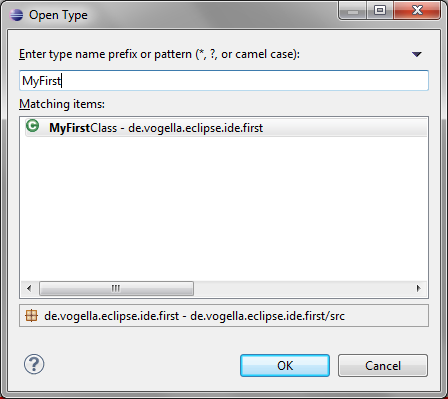
\includegraphics[scale=.5]{images/open-type}
\caption{Отворање класа}
\end{figure}

\subsection{Генерирање код}

Eclipse има неколку можности за генерирање код за вас. Ова може да ви заштеди
значително време при развој.

На пример Eclipse може да ги препокрие методите од суперкласите и генерира
\texttt{toString()}, \texttt{hashcode()} и \texttt{equals()} методи. Исто така
може да генерира и getter и setter методи за атрибутите во вашата Java класа.

Овие опции може да се најдата во менито Source.

\begin{figure}
\centering
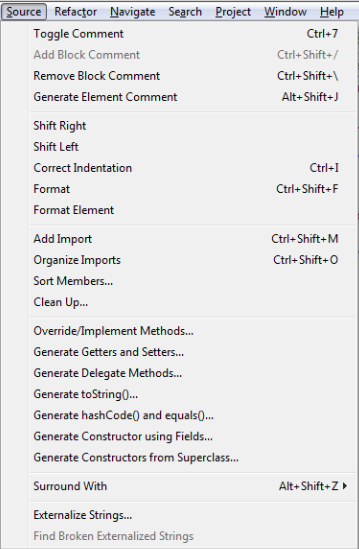
\includegraphics[scale=.5]{images/source}
\caption{Генерирање код}
\end{figure}

За да го тестирање генерирањето на код, ќе ја креираме следната класа во
\texttt{edu.finki.np.first} проектот.

\begin{lstlisting}
package edu.finki.np.first;

public class Person {
  private String firstName;
  private String lastName;

} 
\end{lstlisting}

Изберете Source → Generate Constructor from Fields, маркирајте ги двете
полиња и притиснете ``Ok''.

\begin{figure}
\centering
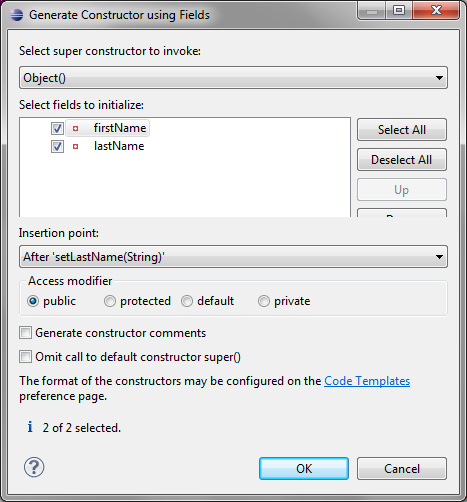
\includegraphics[scale=.5]{images/generate}
\caption{Генерирање}
\end{figure}

Изберете Source → Generate Getter and Setter, изберете ги повторно двете
полиња и притиснете го ``Ok'' копчето.

Изберете Source → Generate toString(), маркирајте ги повторно двете полиња и
притиснете ``Ok''.

Го генериравте следниот код:

\begin{lstlisting}
package edu.finki.np.first;

public class Person {
  private String firstName;
  private String lastName;

  public Person(String firstName, String lastName) {
    super();
    this.firstName = firstName;
    this.lastName = lastName;
  }

  public String getFirstName() {
    return firstName;
  }

  public void setFirstName(String firstName) {
    this.firstName = firstName;
  }

  public String getLastName() {
    return lastName;
  }

  public void setLastName(String lastName) {
    this.lastName = lastName;
  }

  @Override
  public String toString() {
    return "Person [firstName=" + firstName + ", lastName=" + lastName
        + "]";
  }

} 
\end{lstlisting}
\hyperdef{}{refactoring}{\subsection{Refactoring}\label{refactoring}}

\subsection{Refactoring во Eclipse}

Refactoring is the process of restructuring the code without changing
his behavior. For example renaming a Java class or method is a
refactoring activity.

Eclipse supports simple refactoring activities, for example renaming or
moving. For example you can select your class, right click on it and
select Refactor → Rename to rename your class or method. Eclipse will
make sure that all calls in your Workspace to your your class or method
will also be renamed.

The following shows a screenshot for calling the Rename refactoring on a
class.

\begin{figure}[htbp]
\centering
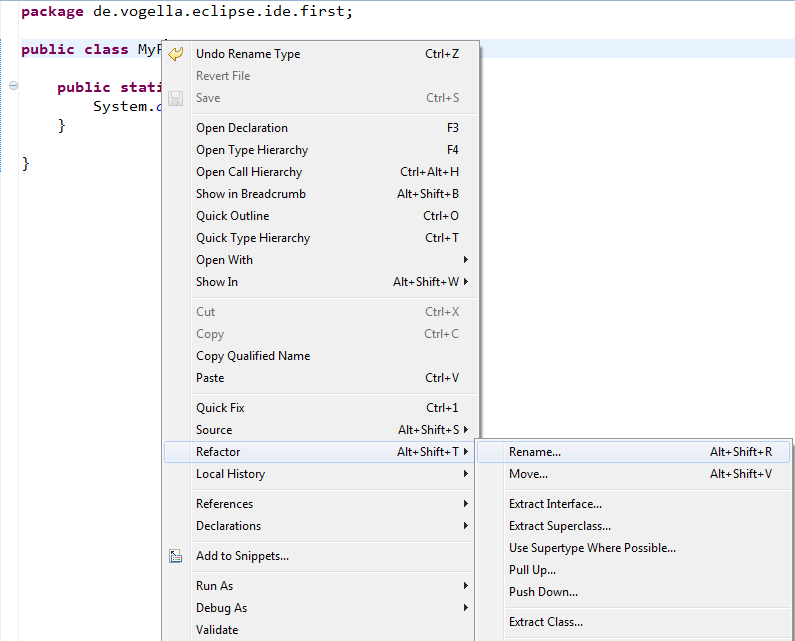
\includegraphics[scale=.5]{images/refactor}
\caption{Renaming a class}
\end{figure}

\subsection{Refactoring Examples}

For the next examples change the code of your \texttt{MyFirstClass}
class to the following.

\begin{verbatim}
package de.vogella.eclipse.ide.first;

public class MyFirstClass {

  public static void main(String[] args) {
    System.out.println("Hello Eclipse!");
    int sum = 0;
    for (int i = 0; i <= 100; i++) {
      sum += i;
    }
    System.out.println(sum);
  }
} 
\end{verbatim}
Another useful refactoring is to mark code and create a method from the
selected code. For this mark the coding of the ``for'' loop, right click
and select Refactoring → Extract Method. Use ``calculateSum'' as name of
the new method.

\begin{figure}[htbp]
\centering
\includegraphics[scale=.5]{images/extract-method}
\caption{Extract Method refactoring}
\end{figure}

The resulting class should look like the following.

\begin{lstlisting}
package de.vogella.eclipse.ide.first;

public class MyFirstClass {

  public static void main(String[] args) {
    System.out.println("Hello Eclipse!");
    int sum = 0;
    sum = calculateSum(sum);
    System.out.println(sum);
  }

  private static int calculateSum(int sum) {
    for (int i = 0; i <= 100; i++) {
      sum += i;
    }
    return sum;
  }
} 
\end{lstlisting}

You can also extract strings and create constants from them. Mark for
this example ``Hello Eclipse!'', right click on it and select Refactor →
Extract Constant. Name your new constant ``HELLO''.

\begin{figure}[htbp]
\centering
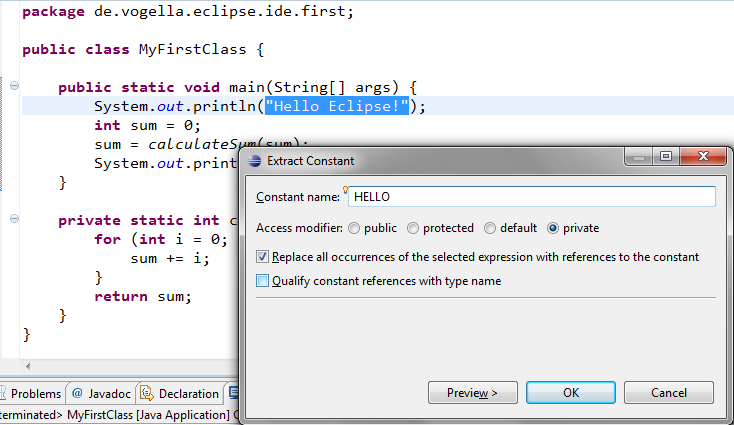
\includegraphics[scale=.5]{images/constants}
\caption{Extract Constants}
\end{figure}

The resulting class should look like the following.

\begin{lstlisting}
package de.vogella.eclipse.ide.first;

public class MyFirstClass {

  private static final String HELLO = "Hello Eclipse!";

  public static void main(String[] args) {
    System.out.println(HELLO);
    int sum = 0;
    sum = calculateSum(sum);
    System.out.println(sum);
  }

  private static int calculateSum(int sum) {
    for (int i = 0; i <= 100; i++) {
      sum += i;
    }
    return sum;
  }
} 
\end{lstlisting}

Eclipse has much more refactorings, in most cases you should get an idea
of the performed action by the naming of the refactoring operation.

\section{Eclipse Shortcuts}

Eclipse provides a lot of shortcuts to work efficiently with the IDE.
For a list of the most important Eclipse shortcuts please see
\href{http://www.vogella.com/articles/EclipseShortcuts/article.html}{Eclipse
Shortcuts}

\section{Using jars (libraries)}

\subsection{Adding a library (.jar) to your project}

The following describes how to add Java libraries to your project. Java
libraries are distributed via ``jar'' files. It assumes that you have a
jar file available; if not feel free to skip this step.

Create a new Java project \texttt{de.vogella.eclipse.ide.jars}. Then,
create a new folder called \texttt{lib}, by right clicking on your
project and selecting New → Folder.

\begin{figure}[htbp]
\centering
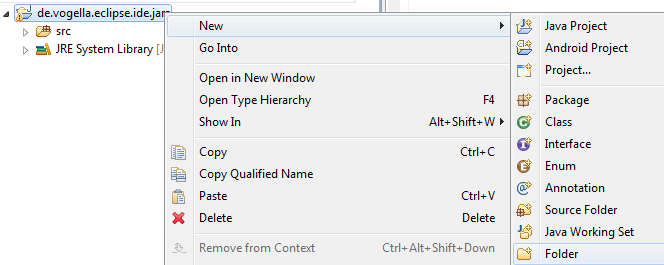
\includegraphics[scale=.5]{images/folder}
\caption{Creating a new folder}
\end{figure}

From the menu select File → Import → General → File System. Select your
jar and select the \texttt{lib} folder as target. Alternatively, just
copy and paste your \texttt{jar} file into the \texttt{lib} folder.

Right click on your project and select Properties. Under Java Build Path
→ Libraries select the Add JARs button.

The following example shows how the result would look like, if the
\texttt{junit-4.4.jar} file had been added to the project.

\begin{figure}[htbp]
\centering
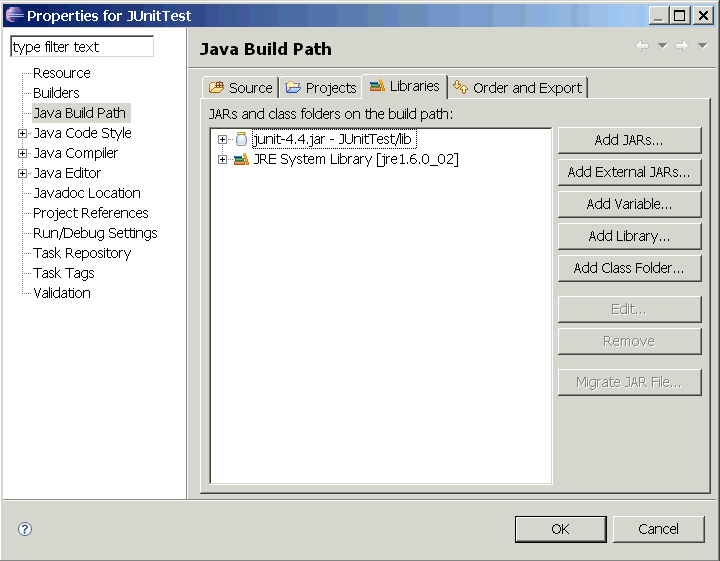
\includegraphics[scale=.5]{images/build-path}
\caption{Adding a jar to the current project}
\end{figure}

Afterwards you can use the classes contained in the \texttt{jar} file in
your Java source code.

\subsection{Attach source code to a Java library}

As said earlier you can open any class via positioning the cursor on the
class in an editor and pressing \textbf{F3}. Alternatively, you can
press \textbf{Ctrl}+\textbf{Shift}+\textbf{T}. This will show a dialog
in which you can enter the class name to open it.

If the source code is not available, the editor will show the decompiled
bytecode of that class.

This happens if you open a class from Java library and the source for
this .jar file is not available. The same happens if you open a class
from the standard Java library without attaching the source code to it.

To browse the source of a type contained in a library (i.e. .jar file),
you can attach a source archive or source folder to that library.
Afterwards the editor will show the source instead of the bytecode.

In addition setting the source attachment allows debugging this source
code.

The Source Attachment dialog can be reached in the Java Build Path page
of a project. To open this page, right click on a project → Properties →
Java Build Path. On the Libraries tab, expand the library's node, select
the Source attachment attribute and press the Edit button.

In the Location path field, enter the path of an archive or a folder
containing the source.

The following shows this for the standard Java library. If you have the
Java Development Kit (JDK) installed, you should find the source in the
JDK installation folder. The file is typically called \texttt{src.zip}.

\begin{figure}[htbp]
\centering
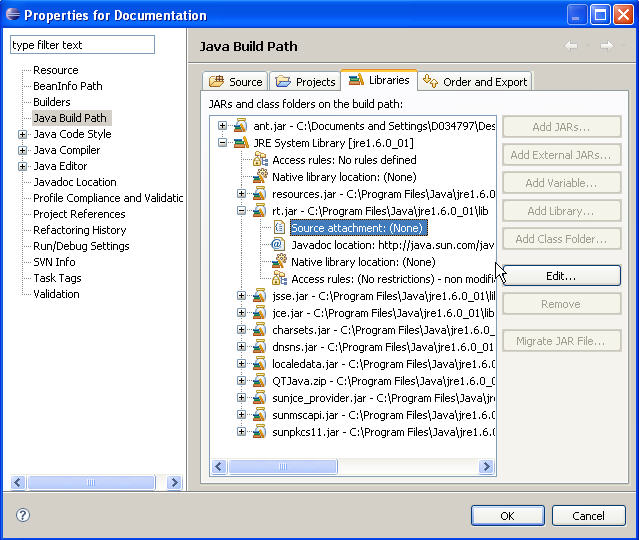
\includegraphics[scale=.5]{images/attach}
\caption{Maintaining the location of the source attachment to an jar}
\end{figure}

\subsection{Add the Javadoc for a jar}

It is also possible to add Javadoc to a library which you use.

Download the Javadoc of the jar and put it somewhere in your filesystem.

Open the Java Build Path page of a project via Right click on a project
→ Properties → Java Build Path. On the Libraries tab expand the
library's node, select the \emph{\texttt{Javadoc location}} attribute
and press the Edit button.

Enter the location to the file which contains the Javadoc.

\begin{figure}[htbp]
\centering
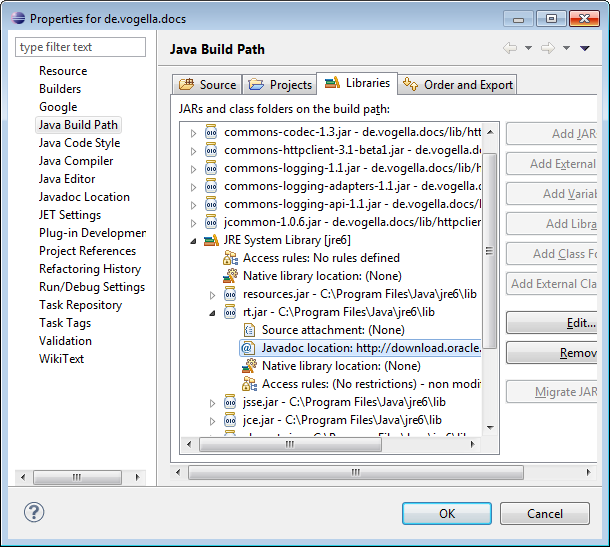
\includegraphics[scale=.5]{images/javadoc}
\caption{Maintain the location to the Javadoc file for a jar file}
\end{figure}

\end{document}
